%++++++++++++++++++++++++++++++++++++++++
% Don't modify this section unless you know what you're doing!
\documentclass[letterpaper,12pt]{article}
\usepackage{tabularx} % extra features for tabular environment
\usepackage{amsmath}  % improve math presentation
\usepackage{graphicx} % takes care of graphic including machinery
\usepackage[margin=1in,letterpaper]{geometry} % decreases margins
\usepackage{cite} % takes care of citations
\usepackage[final]{hyperref} % adds hyper links inside the generated pdf file
\hypersetup{
	colorlinks=true,       % false: boxed links; true: colored links
	linkcolor=blue,        % color of internal links
	citecolor=blue,        % color of links to bibliography
	filecolor=magenta,     % color of file links
	urlcolor=blue         
}
\usepackage{tikz}
%++++++++++++++++++++++++++++++++++++++++


\begin{document}

\title{Physical Education 77: Virtual Fitness}
\date{Location: The Big C || Time: 4-7 Fridays }
\author{Instructors: Emily Harari, Loren Curry, Rachel Elia, Melissa Constantino}
\maketitle

\section{General Information}
In this DeCal, we will work to improve physical fitness, endurance, and respiratory strength through fun and engaging workouts. Our daily warm up will be the walk to the top of the Big C, and from there we will engage in different workout programs such as Just Dance, Wii Sports, and other virtual fitness games and programs. Students will learn a variety of fitness techniques in class that they can apply to their everyday fitness schedule. By the end of this course, students will have a large knowledge of workouts to improve their own fitness, as is the goal of the Physical Education program at UC Berkeley.  


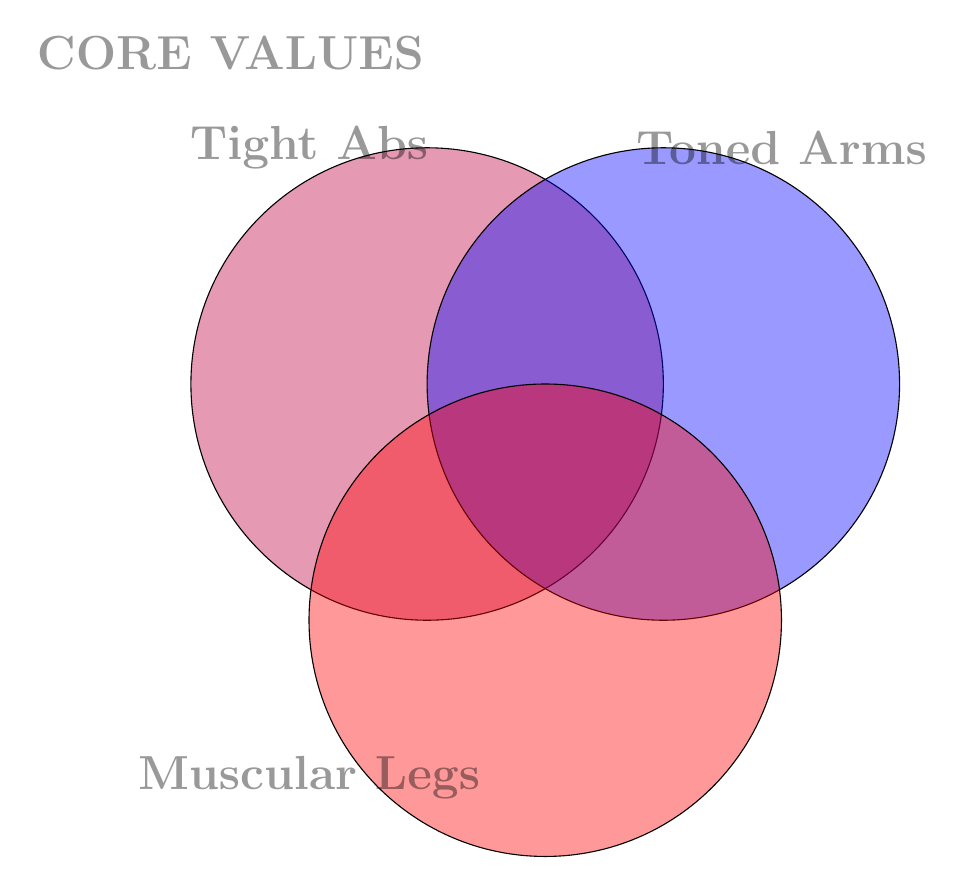
\begin{tikzpicture}
	\begin{scope} [fill opacity = .4]
    \draw[fill=purple, draw = black] (-1.5,1) circle (3);
    \draw[fill=blue, draw = black] (1.5,1) circle (3);
    \draw[fill=red, draw = black] (0,-2) circle (3);
    \node at (-4,5.2) {\LARGE\textbf{CORE VALUES}};
    \node at (-3,4) {\LARGE\textbf{Tight Abs}};
    \node at (3,4) {\LARGE\textbf{Toned Arms}};
    \node at (-3,-4) {\LARGE\textbf{Muscular Legs}};
    \end{scope}
\end{tikzpicture}

\section{Course Requirements and Policies}

All students must have a fun and positive attitude toward trying new things. There are no prior pre-requisites necessary to take this course.

Required Reading: The 4-Hour Body by Tim Ferriss


Add stuff about attendance, technology in class, academic honesty, plagarism, etc. 


\section{Grading}
\begin{table}[ht]
\begin{center}
\caption{Grade Distribution}
\label{tbl:bins} % spaces are big no-no withing labels
\begin{tabular}{|cc|} 
\hline
\multicolumn{1}{|c}{Assignments} & \multicolumn{1}{c|}{Percentage} \\
\hline
Attendance &   30\% \\
Workout Project &   20\% \\
Attitude and Enthusiasm &   0.0018642 \\
Physical Test &   0.0013287 \\
\hline
\end{tabular}
\end{center}
\end{table}





\section{Procedures}

Give a schematic of the experimental setup(s) used in the experiment (see
either in the figure caption or in the text. Write a description of what is
going on. 

Don't forget to list all important steps in your experimental procedure!

Use active voice either in past or present through all the report and be
consistent with it:
The laser light comes  from to ... and eventually arrived to the
balanced photodiode as seen in the figure~\ref{fig:samplesetup}.

Sentences in the past voice while correct are generally considered hard to read
in large numbers. The laser light was directed to ..., wave plates were set
to ... etc.


\section{Analysis}

In this section you will need to show your experimental results. Use tables and
graphs when it is possible. Table~\ref{tbl:bins} is an example.

\begin{table}[ht]
\begin{center}
\caption{Every table needs a caption.}
\label{tbl:bins} % spaces are big no-no withing labels
\begin{tabular}{|cc|} 
\hline
\multicolumn{1}{|c}{$x$ (m)} & \multicolumn{1}{c|}{$V$ (V)} \\
\hline
0.0044151 &   0.0030871 \\
0.0021633 &   0.0021343 \\
0.0003600 &   0.0018642 \\
0.0023831 &   0.0013287 \\
\hline
\end{tabular}
\end{center}
\end{table}

Analysis of equation~\ref{eq:aperp} shows ...

Note: this section can be integrated with the previous one as long as you
address the issue. Here explain how you determine uncertainties for different
measured values. Suppose that in the experiment you make a series of
measurements of a resistance of the wire $R$ for different applied voltages
$V$, then you calculate the temperature from the resistance using a known
equation and make a plot  temperature vs. voltage squared. Again suppose that
this dependence is expected to be linear~\cite{Cyr}, and the proportionality coefficient
is extracted from the graph. Then what you need to explain is that for the
resistance and the voltage the uncertainties are instrumental (since each
measurements in done only once), and they are $\dots$. Then give an equation
for calculating the uncertainty of the temperature from the resistance
uncertainty. Finally explain how the uncertainty of the slop of the graph was
found (computer fitting, graphical method, \emph{etc}.)

If in the process of data analysis you found any noticeable systematic
error(s), you have to explain them in this section of the report.

It is also recommended to plot the data graphically to efficiently illustrate
any points of discussion. For example, it is easy to conclude that the
experiment and theory match each other rather well if you look at
Fig.~\ref{fig:samplesetup} and Fig.~\ref{fig:exp_plots}.

\begin{figure}[ht] 
  \centering
      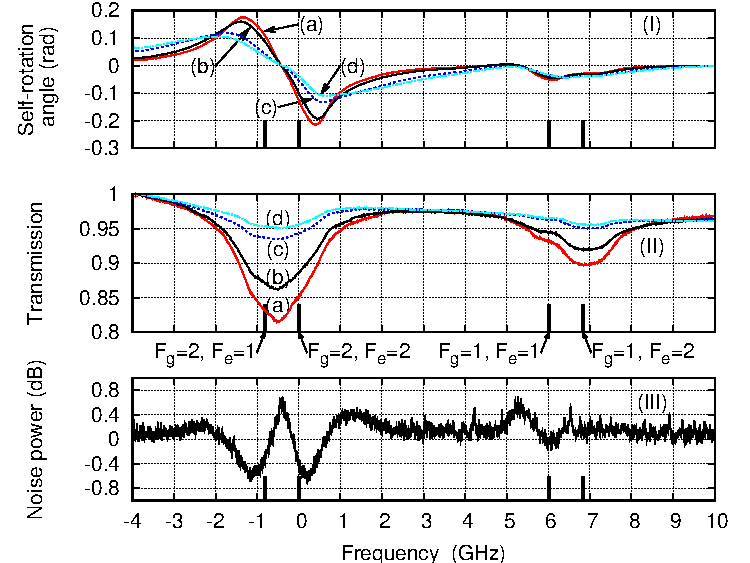
\includegraphics[width=0.5\columnwidth]{sr_squeezing_vs_detuning}

% some figures do not need to be too wide
        \caption{
                \label{fig:exp_plots}  
                Every plot must have axes labeled.
        }
\end{figure}


\section{Conclusions}
Here you briefly summarize your findings.

%++++++++++++++++++++++++++++++++++++++++
% References section will be created automatically 
% with inclusion of "thebibliography" environment
% as it shown below. See text starting with line
% \begin{thebibliography}{99}
% Note: with this approach it is YOUR responsibility to put them in order
% of appearance.

\begin{thebibliography}{99}

\bibitem{melissinos}
A.~C. Melissinos and J. Napolitano, \textit{Experiments in Modern Physics},
(Academic Press, New York, 2003).

\bibitem{Cyr}
N.\ Cyr, M.\ T$\hat{e}$tu, and M.\ Breton,
% "All-optical microwave frequency standard: a proposal,"
IEEE Trans.\ Instrum.\ Meas.\ \textbf{42}, 640 (1993).

\bibitem{Wiki} \emph{Expected value},  available at
\texttt{http://en.wikipedia.org/wiki/Expected\_value}.

\end{thebibliography}


\end{document}
